\section{问题分析}

\subsection{总体思路}

四个问题不是四个独立的建模任务，而是一条串联的流水线：问题一把原始质量信号压缩成一个可比较的标量 $Q$ 并把配比 $p$ 与损失挂钩；问题二把 $Q$ 与 $p$ 嵌进标度律，使``质量''具备与``规模''可换算的量纲；问题三在此损失函数上施加算力预算约束求最优配置；问题四再把损失翻译成可观测的 Benchmark 能力，回答能力增长从何而来。本文的技术路线如图~\ref{fig:roadmap} 所示，研究框架如图~\ref{fig:framework} 所示。

\begin{figure}[htbp]
\centering
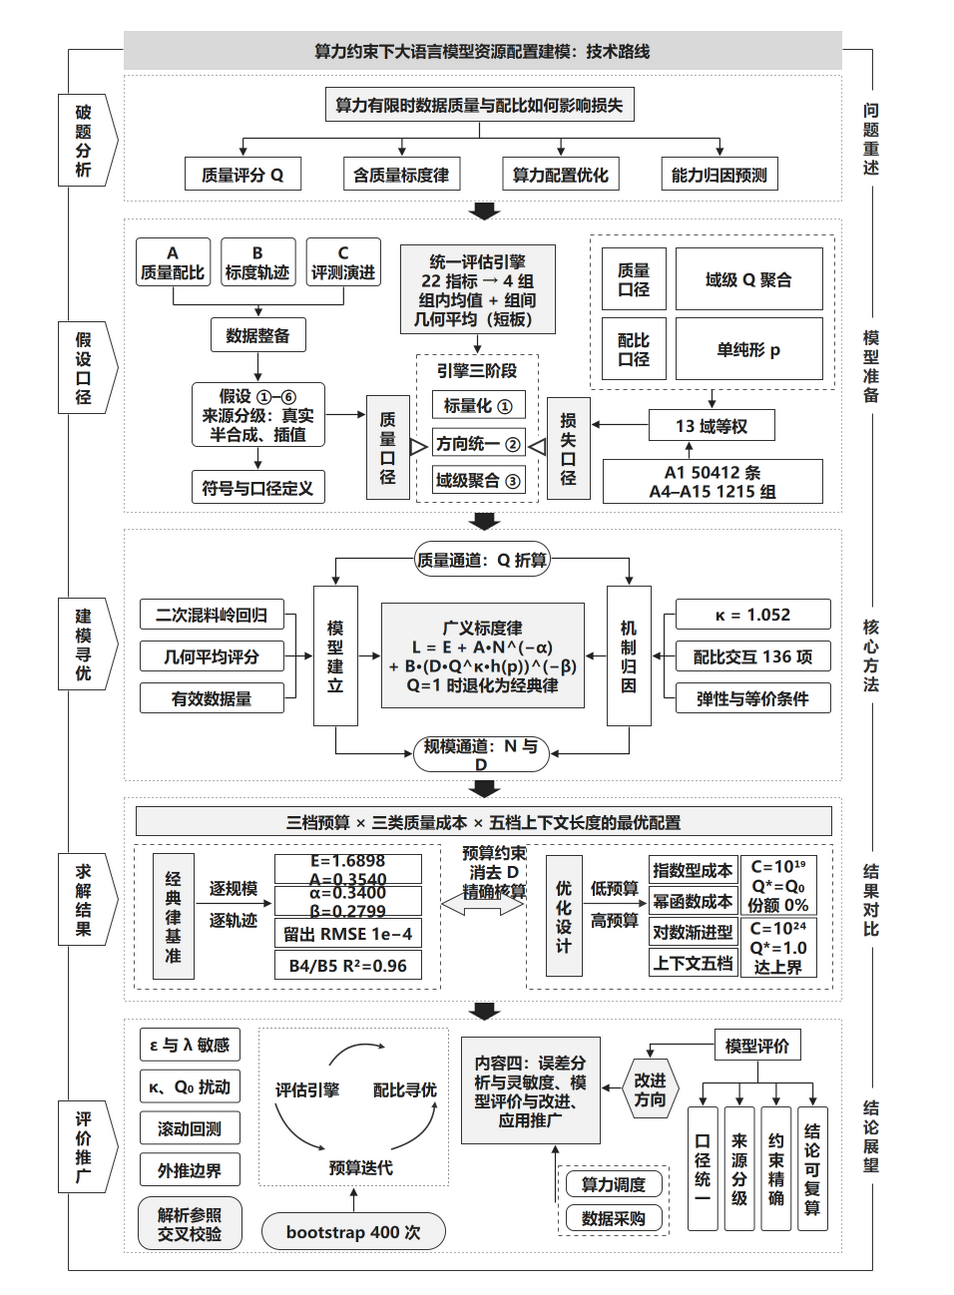
\includegraphics[width=0.86\textwidth]{figures/fig_roadmap.png}
\caption{全文技术路线}
\label{fig:roadmap}
\end{figure}

\begin{figure}[htbp]
\centering
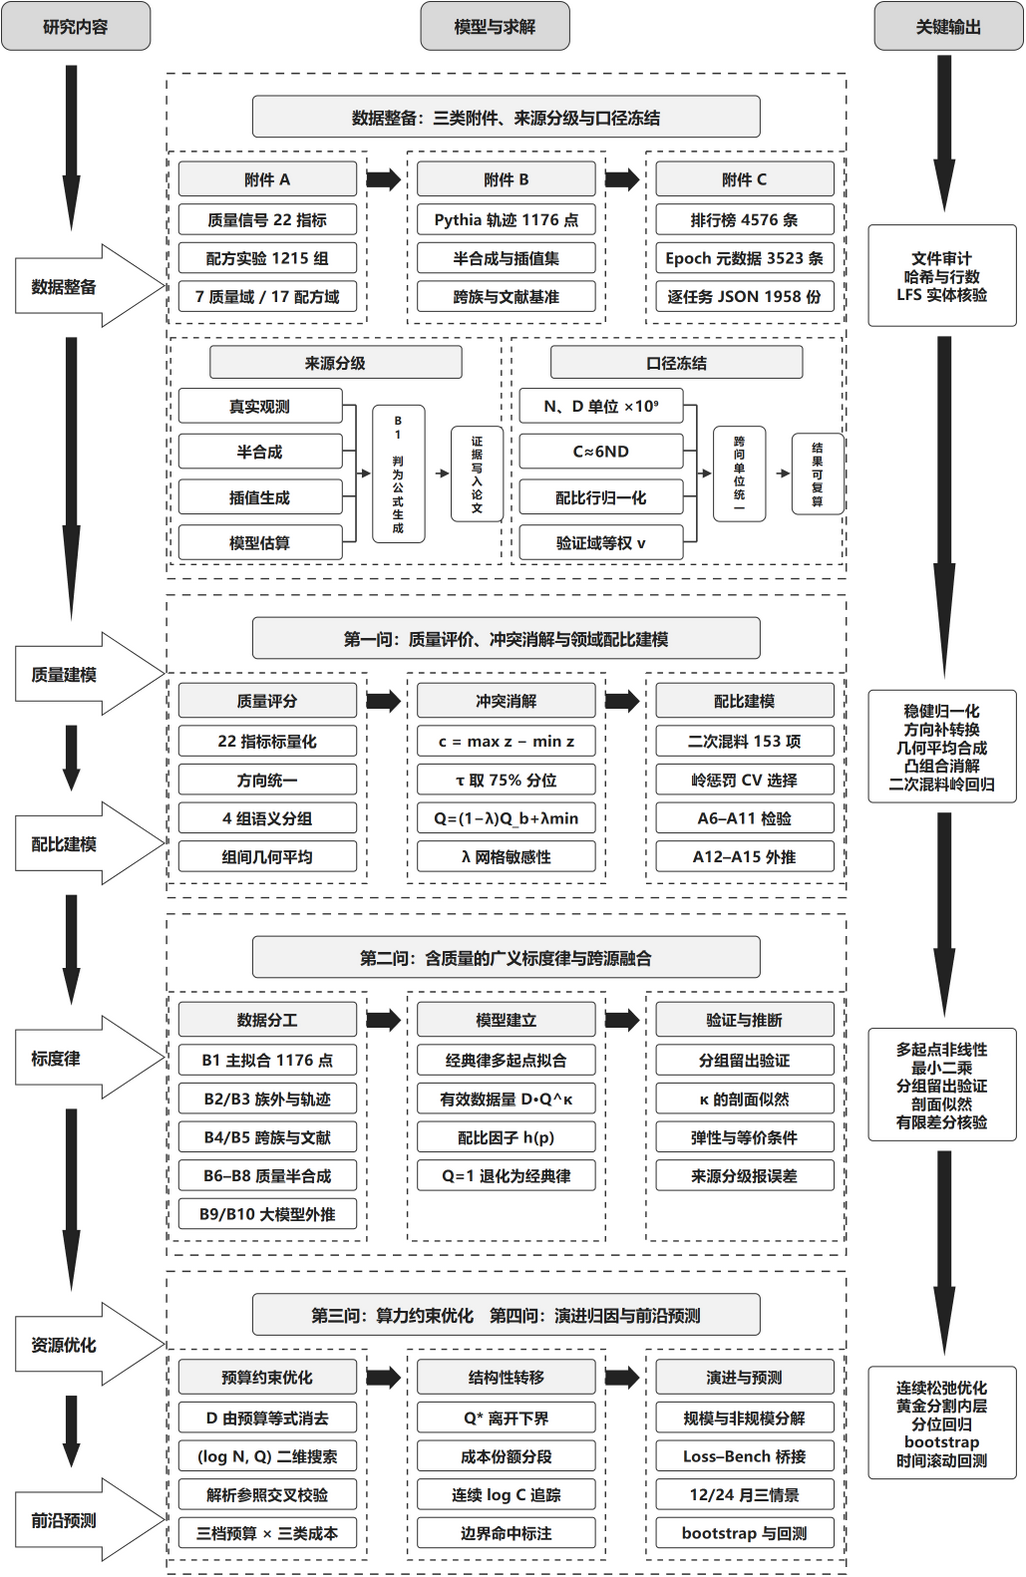
\includegraphics[width=0.92\textwidth]{figures/fig_framework.png}
\caption{研究框架与各问的方法、输出对应关系}
\label{fig:framework}
\end{figure}

贯穿全文的一条纪律是\textbf{来源分级}。题面附件中既有直接观测的真实数据，也有明确标注的半合成、插值与估算数据；若不加区分地混用，很容易把``生成数据的规律''误当成``真实世界的规律''。因此本文对每份数据先做可解释性诊断，再决定它在模型中的角色，并在结果中区分报告。

\subsection{问题一分析}

本问要回答三件事，它们的技术难点各不相同。

\textbf{质量评分}的难点在于 22 个指标语义与量纲都不统一：其中 8 个是多维列表（如 \texttt{modernbert\_*} 是六分类 logits、\texttt{qurater} 是四维子分、\texttt{ad\_en} 是二分类 logits），必须先压缩成标量；而 \texttt{rps\_doc\_word\_count} 这类指标并非单调越好，过短过长都不理想，机械规定方向会引入偏差。本文的处理是先按语义分组，再在组内平均、组间做几何平均——几何平均对短板敏感，恰好对应``教材某一维度很差会拖累整体''的直觉。

\textbf{质量冲突}需要先给出可计算的定义。两组指标对同一文本给出显著不一致的评价时，最直观的度量是各组得分之间的极差 $c=\max_g z_g-\min_g z_g$。但``不一致''不等于``某一方错了''：教材信息量大而排版不规范是真实存在的特征，因此消解规则应当保留这一信息而非简单取平均。本文采用算术平均与最弱组的凸组合，强度 $\lambda$ 由小规模预设网格确定并做敏感性分析。

\textbf{配比建模}的关键是单纯形约束。由于 $\sum_i p_i=1$，完整二次多项式中的截距项与平方项并不独立于一次项，本文采用 Scheffé 规范形，只保留 17 个一次项与 136 个两两交互项。样本量 512 对 153 个参数偏紧，故使用岭惩罚并由交叉验证选择强度。

本问还有一个容易被忽略的陷阱：若把质量引入配比回归，需要注意 $Q(p)=\sum_i p_iq_i$ 本身就是 $p$ 的线性函数，与线性配比项\textbf{完全共线}。本文专门对此做了诊断，结论见\ref{sec:q1_quality_in}节。

\subsection{问题二分析}

\textbf{跨源融合}是本问最大的困难。附件 A 与附件 B 是相互独立的实验，验证集、tokenizer 与损失坐标都不必然一致，不能按行直接拼接。本文的处理分三步：先为每一份数据做``是否落在经典律曲面上''的诊断，判断它能否提供独立的泛化证据；再检验不同来源在基准质量处是否同尺度；最后才做分阶段参数估计。

\textbf{模型形式}上，题面提示``当教材趋于完美时新公式退化为经典形式''。本文采用有效数据量的形式，把质量与配比折算成等效的数据量：

\begin{equation}
L(N,D,Q,p)=E+AN^{-\alpha}+B\left[D\,Q^{\kappa}h(p)\right]^{-\beta},\qquad h(p_0)=1,\ h(p)>0.
\end{equation}

当 $Q=1$ 且 $p=p_0$ 时该式严格退化为经典律。这一形式的好处是 $\kappa$ 有直接解释：$\kappa=1$ 意味着``质量提升 $x$ 倍等价于数据量提升 $x$ 倍''，$\kappa>1$ 则意味着质量的作用被放大。

\textbf{等价条件}的推导要点在于：同等损失改善既可以靠提高 $Q$，也可以靠增大 $N$，但两条路径的代价不同。由 $L$ 对 $N$ 的幂律形式可以解析解出``质量提升 $\Delta Q$ 所等效的规模增量''，但必须注意该式只在括号内为正时有有限解——括号归零意味着需要无限规模，为负则意味着单靠增大 $N$ 根本无法实现同等收益。

\subsection{问题三分析}

本问是带约束的非线性优化。三个成本项共用同一个 $D$，因此预算约束可整理为

\begin{equation}
D\left\{(6+\eta\ell)N+[g(Q)-g(Q_0)]_+\right\}\le C .
\end{equation}

由于损失对 $D$ 单调下降且题面未给出数据量上限，最优点处预算必然紧约束，于是可解析消去 $D$，把二维搜索降为 $(\log N,Q)$ 上的无约束问题。这一化简的前提必须在实施前检查，本文在\ref{sec:q3_check}节中逐条核验。

需要特别注意的是\textbf{结构性转移的识别}。题面用``家庭收入从 3000 元到 3 万元再到 30 万元''作类比，但仅在三个离散预算点上观察到差异并不足以证明变点存在。本文的做法是：先在连续 $\log C$ 网格上追踪最优解，再用解析参照与一阶条件确认数值解正确，最后检查观察到的变化是否在参数扰动下稳定复现。

另有一个理论上的结论需要预先说明：在本题的算力代理下，固定 $\ell$ 时注意力开销与训练开销之比 $C_{\mathrm{attn}}/C_{\mathrm{train}}=\eta\ell/6$ 是常数，因此\textbf{两者的份额之比本身不会随预算产生结构转移}。真正可能发生转移的是质量投入的存在性与强度。

\subsection{问题四分析}

本问的第一个难点是\textbf{口径统一}：``能力''用哪个综合分、``开源''如何筛选、``时间''按提交日期还是发布日期、模型类型如何区分``预训练''与``对话微调''。这些口径不统一，后续的贡献分解就无从谈起。

第二个难点是\textbf{避免重复计入}。数据工程带来的收益已经在 $Q$ 与 $p$ 中被解释过一次，若在时间趋势项里再完整计入一遍，就会高估技术进步。本文的做法是把时间项解释为``控制规模与类型后仍存在的剩余趋势''，并在正文中如实说明它还可能包含评测口径变化等遗漏因素，不把它称作因果效应。

第三个难点是\textbf{组成变化}。若直接用季度平均能力做分解，会受``提交的模型越来越小''这一组成变化污染——本文的数据确实显示季度平均参数量在下降。因此主分解建立在固定组成子集上，并另做分位数前沿的对照分解。

最后，Loss 与 Benchmark 之间的\textbf{桥接}本身误差很大（本文实测留一 MAE 达 7.34 分），必须把这一不确定性显式传播到预测区间中，而不是给一个看似精确的点预测。
